%=============================================================================%
% Preamble
%=============================================================================%
% Libraries

\documentclass[xcolor=table,aspectratio=169]{beamer}
%\usepackage{beamerthemeshadow}
\usepackage{helvet}
\usepackage[]{graphicx}
\usepackage{array}
\usepackage{color}
\definecolor{dkgreen}{rgb}{0,0.6,0}
\definecolor{gray}{rgb}{0.5,0.5,0.5}
\definecolor{mauve}{rgb}{0.58,0,0.82}
\definecolor{deepblue}{rgb}{0,0,0.5}
\definecolor{deepred}{rgb}{0.6,0,0}
\definecolor{deepgreen}{rgb}{0,0.5,0}
\definecolor{lightgray}{rgb}{0.92,0.92,0.92}
\usepackage{listings} % to insert code
\usepackage{textpos} % textblock
\usepackage{hyperref}
\hypersetup{colorlinks=true, urlcolor=blue, linkcolor=black} 
% Listing set up
% bash
\lstdefinestyle{bash}{
language=bash,                     % the language of the code
basicstyle=\scriptsize\ttfamily,       % the size of the fonts that are used for the code
numbers=none,%left,                   % where to put the line-numbers
numberstyle=\tiny\color{gray},  % the style that is used for the line-numbers
stepnumber=1,                   % the step between two line-numbers. If it's 1, each line
                          % will be numbered
numbersep=5pt,                  % how far the line-numbers are from the code
backgroundcolor=\color{lightgray},  % choose the background color. You must add \usepackage{color}
showspaces=false,               % show spaces adding particular underscores
showstringspaces=false,         % underline spaces within strings
showtabs=false,                 % show tabs within strings adding particular underscores
frame=lines,%single,                   % adds a frame around the code
rulecolor=\color{black},        % if not set, the frame-color may be changed on line-breaks within not-black text (e.g. commens (green here))
tabsize=2,                      % sets default tabsize to 2 spaces
captionpos=b,                   % sets the caption-position to bottom
breaklines=true,                % sets automatic line breaking
breakatwhitespace=false,        % sets if automatic breaks should only happen at whitespace
title=\lstname,                 % show the filename of files included with \lstinputlisting;
                          % also try caption instead of title
keywordstyle=\color{blue},      % keyword style
commentstyle=\color{dkgreen},   % comment style
stringstyle=\color{mauve},      % string literal style
escapeinside={\%*}{*)},         % if you want to add a comment within your code
morekeywords={}            % if you want to add more keywords to the set
}

\lstdefinestyle{python}{
language=python,
formfeed=\newpage,
basicstyle=\scriptsize\ttfamily,
commentstyle=\color{deepgreen},%\color{gray},
numbers=left,
numberstyle=\tiny\color{gray},
stepnumber=1,
numbersep=5pt,
backgroundcolor=\color{lightgray},%\color{white},
showspaces=false,
showstringspaces=false,
showtabs=false,
frame=lines,
tabsize=4,
captionpos=b,
breaklines=true,
breakatwhitespace=false,
title=\lstname,
escapeinside={},
keywordstyle=\color{deepblue},
emphstyle=\color{deepred},
stringstyle=\color{deepgreen}
%morekeywords={models, lambda, forms}
}

\graphicspath{ {../img/} }

\begin{document}
\title{Programming in Python for Scientific Research}   
\subtitle{Introduction to Python}   
\author{Bram Kuijper}
\institute[]{University of Exeter, Penryn Campus, UK}
\date{}
\titlegraphic{
\hfill

\includegraphics[width=\textwidth, keepaspectratio]{IDSAI.pdf}}

\frame{\titlepage} 
\begin{frame}{Acknowledgements}
\begin{itemize}\addtolength{\itemsep}{\baselineskip}
    \item This course is funded by UExeter's Institute for Data Science and Artificial Intelligence: \href{https://www.exeter.ac.uk/idsai/}{IDSAI}
    \item This course was originally designed by the late and great JJ Valletta (1983 - 2020), who worked as a postdoc here in Penryn
\begin{center}
    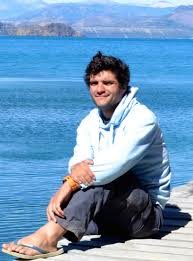
\includegraphics[width = 20mm]{jj_valletta.jpg}
\end{center}
\end{itemize}
%
\includegraphics[width=\textwidth, keepaspectratio]{logo.jpg}

\end{frame}

\frame{\frametitle{Intended learning outcomes}
\begin{itemize}
    \item Know how to access resources and learning materials on Python
        \pause
    \item Understand pros and cons of choosing Python as a programming language
        \pause
    \item Find your Python distribution of choice
        \pause
    \item Understand how to run Python on your computer
\end{itemize}
        \pause
\emph{Slides provide various \href{https://docs.python.org/3/}{pointers} to further information}
}

\frame{\frametitle{Resources for self-study}
\begin{itemize}
    \item Course website \url{https://exeter-data-analytics.github.io}
        \begin{itemize}
            \item Lecture slides and videos
            \item Exercises
            \item Additional resources
        \end{itemize}
        \pause
    \item Python documentation: \url{https://docs.python.org}
        \begin{itemize}
            \item They have a \href{https://docs.python.org/3/tutorial/index.html}{pretty good tutorial}, particularly for those who already have some programming experience
        \end{itemize}
\end{itemize}
}

\frame{\frametitle{Resources for self-study II: some of many books}
\begin{columns}
\column{0.33\textwidth}
    \begin{minipage}[c][0.6\textheight][c]{\linewidth}
        \centering
        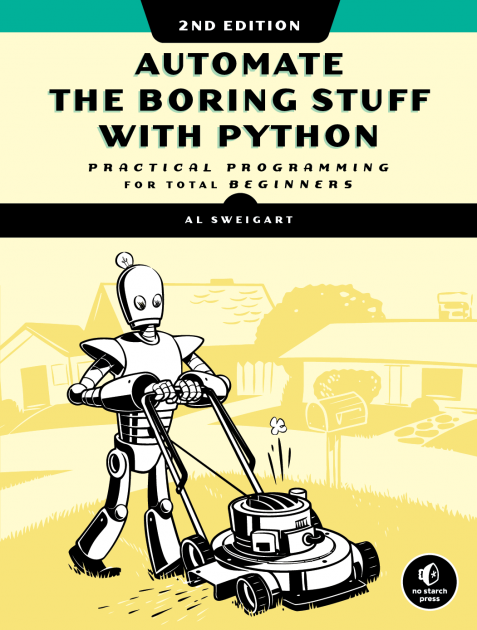
\includegraphics[width=0.8\linewidth]{automate_2e_cover.png}
    \end{minipage}
    \begin{minipage}[c][0.2\textheight][c]{\linewidth}
        \small{very practical intro on Python: e.g., working with many files, interacting with Excel/Word/PDF documents, GUI automation. Free online} 
    \end{minipage}

% 2nd column
\column{0.33\textwidth}
    \begin{minipage}[c][0.6\textheight][c]{\linewidth}
        \centering
        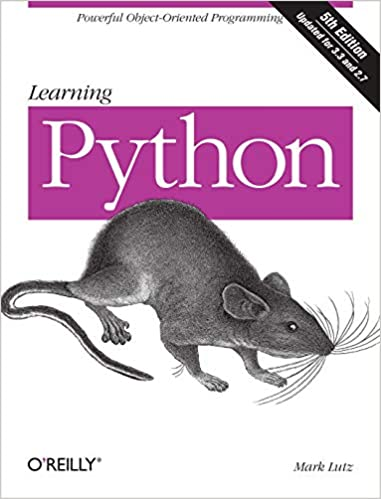
\includegraphics[width=0.8\linewidth]{lutz_python.png}
    \end{minipage}
    \begin{minipage}[c][0.2\textheight][c]{\linewidth}
        \small{Covers everything in detail, hence not a quick introduction. UExeter e-resource} 
    \end{minipage}

%3rd column 
\column{0.33\textwidth}
    \begin{minipage}[c][0.6\textheight][c]{\linewidth}
        \centering
        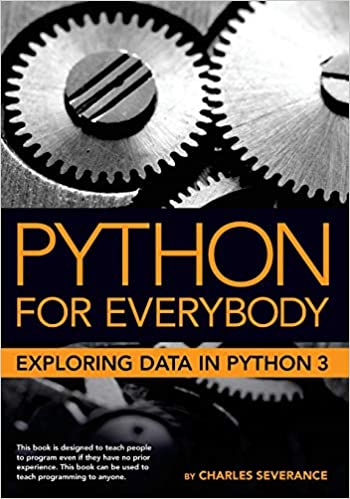
\includegraphics[width=0.8\linewidth]{severance_book.jpg}
    \end{minipage}
    \begin{minipage}[c][0.2\textheight][c]{\linewidth}
        \small{Good balance between detail and basic introduction. Free online} 
    \end{minipage}
\end{columns}
}

\frame{\frametitle{What is Python?}
\begin{itemize}
    \item A scripted, high-level programming language created by \href{https://gvanrossum.github.io/}{Guido Van Rossum} and named after \href{https://en.wikipedia.org/wiki/Monty_Python\%27s_Flying_Circus}{Monty Python's flying circus}
\begin{center}
    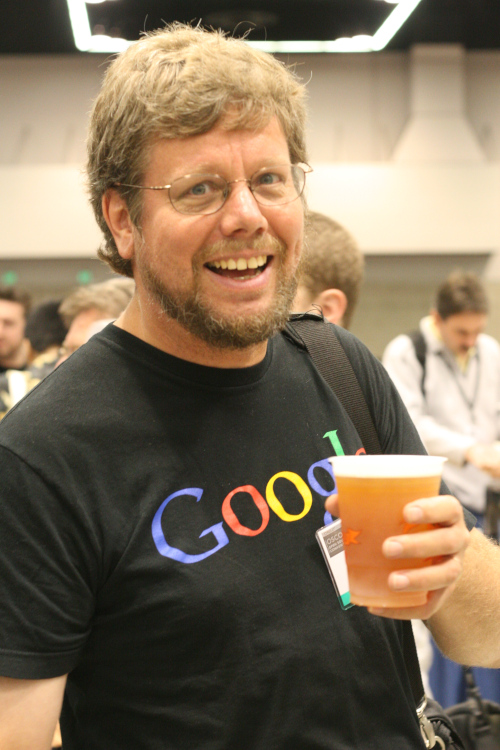
\includegraphics[width = 20mm]{GuidoVanRossumSmall.jpg}
    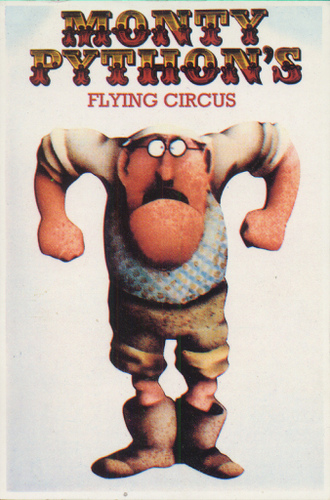
\includegraphics[width = 20mm]{MontyPython.jpg}
\end{center}
    \pause
    \item easy-to-use, highly standardized and with an emphasis on readability of code
\end{itemize}
}

\frame{\frametitle{Why use Python?}
The \href{https://www.tiobe.com/tiobe-index/}{TIOBE} index is a measure of the popularity of programming languages:
    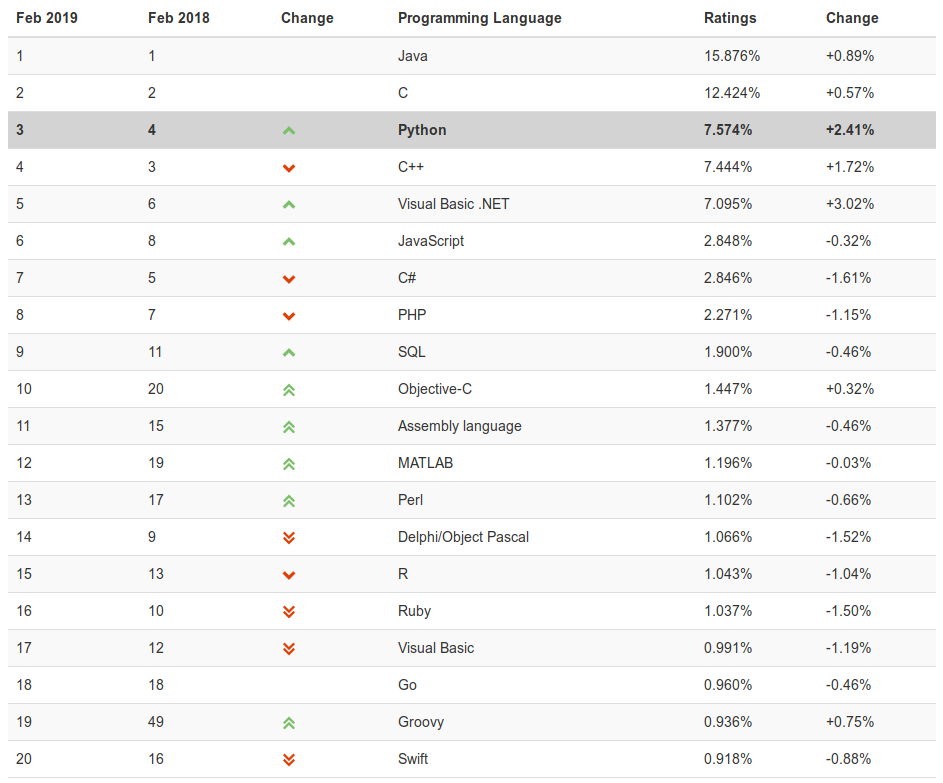
\includegraphics[width = 10cm]{TiobeIndex.png}
}

\begin{frame}{Why Python?}
%. Here are some reasons for its popularity:

\begin{itemize}\addtolength{\itemsep}{0.5\baselineskip}
	\item<1-> It is free! No licence costs
	\item<2-> Runs on almost any platform (Mac, Windows, Linux)
	\item<3-> Because of its ease of programming, Python minimises development effort
	\item<4-> A huge number of \href{https://pypi.python.org/pypi}{libraries}, written by an active \href{https://www.python.org/community/}{community}  
	\item<5-> Python can ``glue" together functions written in C/C++ and Fortran to speed things up (we can also call R and MATLAB functions)
	\item<6-> Compared to other high-level scientific languages such as MATLAB and R, Python offers a much wider range of additional functionality (e.g \href{https://www.djangoproject.com/}{web} and \href{https://wiki.python.org/moin/TkInter}{GUI} development) %hence the nickname ``the swiss army knife" of programming languages. 
\end{itemize}

\end{frame}

%=============================================================================%
%=============================================================================%
\begin{frame}{Horses for courses}

\begin{itemize}\addtolength{\itemsep}{0.5\baselineskip}
        \item<1-> Python is becoming the \emph{de facto} standard for exploratory and interactive scientific research\\
	\item<2-> But, python is no programming silver bullet!!
	\item<3-> Your application will dictate the tool (and a mixture of more than one language is ok). For example:\\
	\begin{itemize}\addtolength{\itemsep}{0.8\baselineskip}
            \item<4-> \href{https://jsommers.github.io/cbook/index.html}{C} and its descendant \href{https://www.stroustrup.com/C++.html}{C++} excel at heavy-duty applications with fast runtimes (but long development times): simulations with lots of calculations, operating systems, web browsers, word processors, ...
            \item<5-> \href{https://uk.mathworks.com/help/matlab/}{MATLAB} excels at interfacing with hardware, e.g generating \href{https://uk.mathworks.com/products/hdl-coder.html}{hardware description language (HDL) code} to configure an integrated circuit board or connecting to a \href{https://uk.mathworks.com/products/daq.html}{data acquisition card}. Caveat is that MATLAB costs \pounds \pounds \pounds
            \item<6-> R excels at data selection, visualisation and statistical modelling (but Python libraries are catching up: \href{https://pandas.pydata.org/docs/user_guide/index.html}{\texttt{pandas}}, \href{https://matplotlib.org/}{\texttt{matplotlib}} and \href{https://www.statsmodels.org/stable/index.html}{\texttt{statsmodels}})
	\end{itemize}
\end{itemize}

\end{frame}


\begin{frame}{Why do \textit{you} want to learn Python?}
    Some reasons:
    \pause
    \begin{itemize}
        \item Python has a simple syntax and is widely used; ideal language for beginners
            \pause
        \item High quality error reporting and debugging tools (compare R/Perl/bash)
            \pause
        \item Development of applications quicker than for compiled languages like C or Java
            \pause
        \item Python (and R) have replaced Perl as the key bioinformatics language
            \pause
        \item GIS applications like ArcGIS use Python as their main scripting language
            \pause
        \item Language of choice for machine learning (PyTorch, scikit, TensorFlow)
    \end{itemize}
\end{frame}

\frame{\frametitle{Python version 2 vs 3}
    \begin{itemize}
        \item Some systems (Mac) still use Python 2 as the default  
            \pause
        \item Python 2 is a legacy version and is now largely replaced by Python 3
            \pause
        \item Python 3 differs in \href{https://sebastianraschka.com/Articles/2014\_python\_2\_3\_key\_diff.html}{various ways} from Python 2
            \pause
        \item Often, Python 3 code cannot be run using a Python 2 interpreter and vice versa
            \pause
        \item \textbf{We will only focus on Python 3}
    \end{itemize}
}

\frame{\frametitle{Different Python distributions}
Various distributions of Python available:
    \begin{itemize}
            \pause
        \item Download official distribution straight from \href{https://python.org}{python.org} 
            \pause
        \item On Mac/Linux, official distribution available through package managers like \texttt{apt-get}, \texttt{yum} or \href{https://installpython3.com/mac/}{homebrew}
            \begin{itemize}
                \item Official distribution requires libraries and IDEs to be installed separately via \href{https://pip.pypa.io/en/stable/}{\texttt{pip} (Python's package manager)}
            \end{itemize}
            \pause
        \item \href{https://www.enthought.com/product/canopy/}{Enthought Canopy}: Python, libraries \& tools in single installer
            \pause
        \item \href{https://www.anaconda.com/distribution/}{Anaconda}: Python, libraries \& tools in single installer: \textbf{used in this course}
            \begin{center}

\includegraphics[width=0.3\textwidth]{AnacondaLogo.png}
            \end{center}
            \pause
        \item Stick to one distribution, otherwise python will \href{https://xkcd.com/1987/}{mix up libraries}
    \end{itemize}
}



\begin{frame}[fragile]
\frametitle{Executing Python code: Spyder IDE}
    \begin{itemize}
        \item Windows: Start Menu $>$ Anaconda3 $>$ Spyder
            \pause
        \item Mac: Applications $>$ Spyder
    \end{itemize}
\end{frame}

\begin{frame}[fragile]
\frametitle{Executing Python code: Spyder IDE}
\begin{itemize}\addtolength{\itemsep}{.7\baselineskip}
	\item Spyder is an integrated development environment (IDE) for scientific computing, akin to \href{https://www.rstudio.com/}{RStudio} and \href{https://uk.mathworks.com/products/matlab.html}{MATLAB} 
        \pause
	\item One place to write, execute and debug code, and explore variables
\end{itemize}

\begin{center}
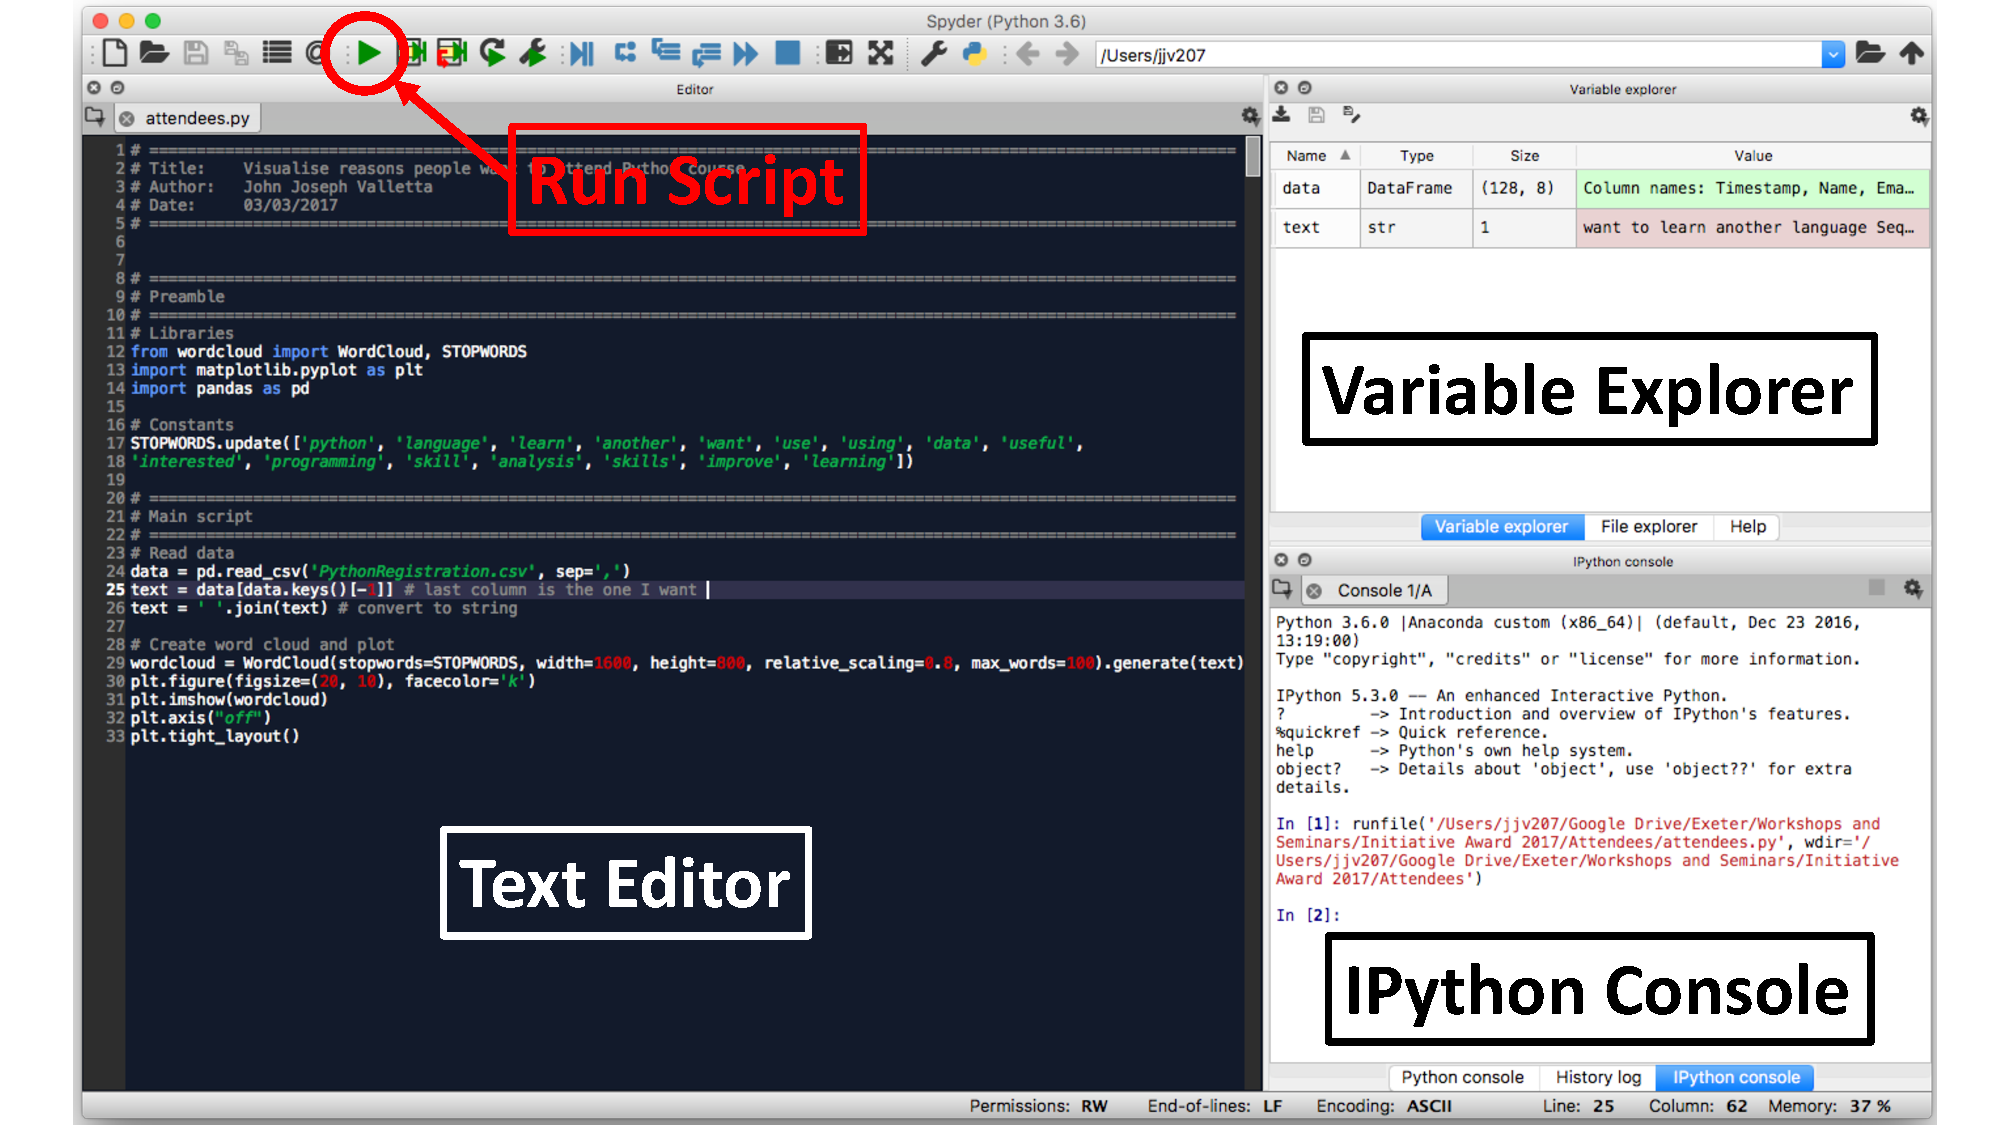
\includegraphics[width=0.8\textwidth]{spyder_annotated.pdf}
\end{center}
\end{frame}

\begin{frame}[fragile]
\frametitle{Running standalone Python scripts without the IDE - I}
Being able to run Python scripts without the Spyder IDE is particularly important when running scripts on computing clusters. 

    
\begin{itemize}
    \item Windows: don't bother, use the Spyder IDE
        \pause
    \item Mac/Linux: 
        \begin{itemize}
            \item Write your code in a plain text file, say \texttt{my\_script.py}
                \pause
            \item In a terminal, run:
\begin{lstlisting}[style=bash]
python3 my_script.py
\end{lstlisting}
\end{itemize}
\end{itemize}

\end{frame}


\begin{frame}[fragile]
\frametitle{Running standalone Python scripts without the IDE - II}
By adding a so-called `shebang' to the top of a Python script, one 
can run scripts as a standalone programme on Mac / Linux \vspace{3pt}
   \pause 
\begin{itemize}\addtolength{\itemsep}{0.05\baselineskip}
    \item Add a shebang \texttt{\#!/usr/bin/env python3}, to the first line of the python script file, here called \texttt{my\_script.py}:
\begin{lstlisting}[style=python]
#!/usr/bin/env python3

print("This Python script prints something.")
...
\end{lstlisting}
    \pause 
    \item Close the file and make it executable by typing in a terminal
\begin{lstlisting}[style=bash]
chmod +x my_script.py
\end{lstlisting}
    \pause 
    \item Run the script by typing in a terminal
\begin{lstlisting}[style=bash]
./my_script.py
This Python script prints something.
\end{lstlisting}
\end{itemize}
\end{frame}




\end{document}

